\chapter{Introduction to Machine Learning}\label{ch-01}

The first lecture has a twofold purpose: to motivate the study of
\textbf{Machine Learning} (ML) by placing it within the landscape of
computer science and artificial intelligence, and to provide practical
information about the course (prerequisites, structure, exam,
materials). At the end, the basic mathematical concepts needed
throughout the course are reviewed.

\section{What is Machine
Learning}\label{che-cosuxe8-il-machine-learning}

\subsection{Learning as a universal
principle}\label{lapprendimento-come-principio-universale}

Learning is a principle shared by living beings, societies and ---
today --- machines. As Poggio and Shelton observe (\emph{AI Magazine},
1999), \emph{the problem of learning is arguably at the very core of the
problem of intelligence, both biological and artificial}. Understanding
how we learn therefore means understanding a fundamental part of what
it means to be intelligent.

\begin{boxdefinition}{Machine Learning}

\textbf{Machine Learning} is a theoretical and applied area of computer
science that combines two goals: the artificial intelligence goal of
building \textbf{computers capable of learning}, and that of having
\textbf{powerful adaptive and statistical tools} with rigorous
foundations in the computational sciences. Operationally, it is the
automatic learning, by a system, from \textbf{experience} (a set of
examples), aimed at solving a computational task.

\end{boxdefinition}

\subsection{Why make machines learn: luxury or
necessity?}\label{perchuxe9-far-apprendere-le-macchine-lusso-o-necessituxe0}

ML is not a technological fad but a \textbf{necessity}, for two main
reasons:

\begin{enumerate}
\def\labelenumi{\arabic{enumi}.}
\tightlist
\item
  \textbf{Growing availability of empirical data} and the need to
  analyse it. Science itself is shifting its paradigm towards a
  \emph{data-driven} approach, in which knowledge is extracted from
  data; ML plays a central, methodological role in this change.
\item
  \textbf{It is hard to explicitly program adaptivity and
  intelligence}. Alan Turing had already realised this: for many tasks
  writing the rules by hand is impractical, and learning becomes the
  only way to endow systems with intelligent behaviour.
\end{enumerate}

The combination of \textbf{large amounts of data}, \textbf{computing
power} (HPC, GPUs) and \textbf{flexibility of ML models} has opened a
new era of artificial intelligence.

\subsection{When ML is needed}\label{quando-serve-il-ml}

ML is the right choice when there is \textbf{little or no prior
knowledge} about a problem (we do not know how to write the rules of the
solution), but it is relatively \textbf{easy to obtain experience}, i.e.
data for which we know the correct result. Classic examples are
classifying emails as \emph{spam}, and recognising characters, faces or
speech.

\begin{boxexample}{Handwritten digit recognition}

Each digit is an \(8 \times 8\) pixel image. Writing by hand the rules
that distinguish a ``3'' from an ``8'' for every possible handwriting
is practically impossible. Instead, many already-labelled examples of
digits are collected and the system is left to \textbf{learn a
classifier} \(f\) that maps each image to the correct class
(\(0, 1, \dots, 9\)).

\end{boxexample}

\begin{figure}[htbp]
\centering
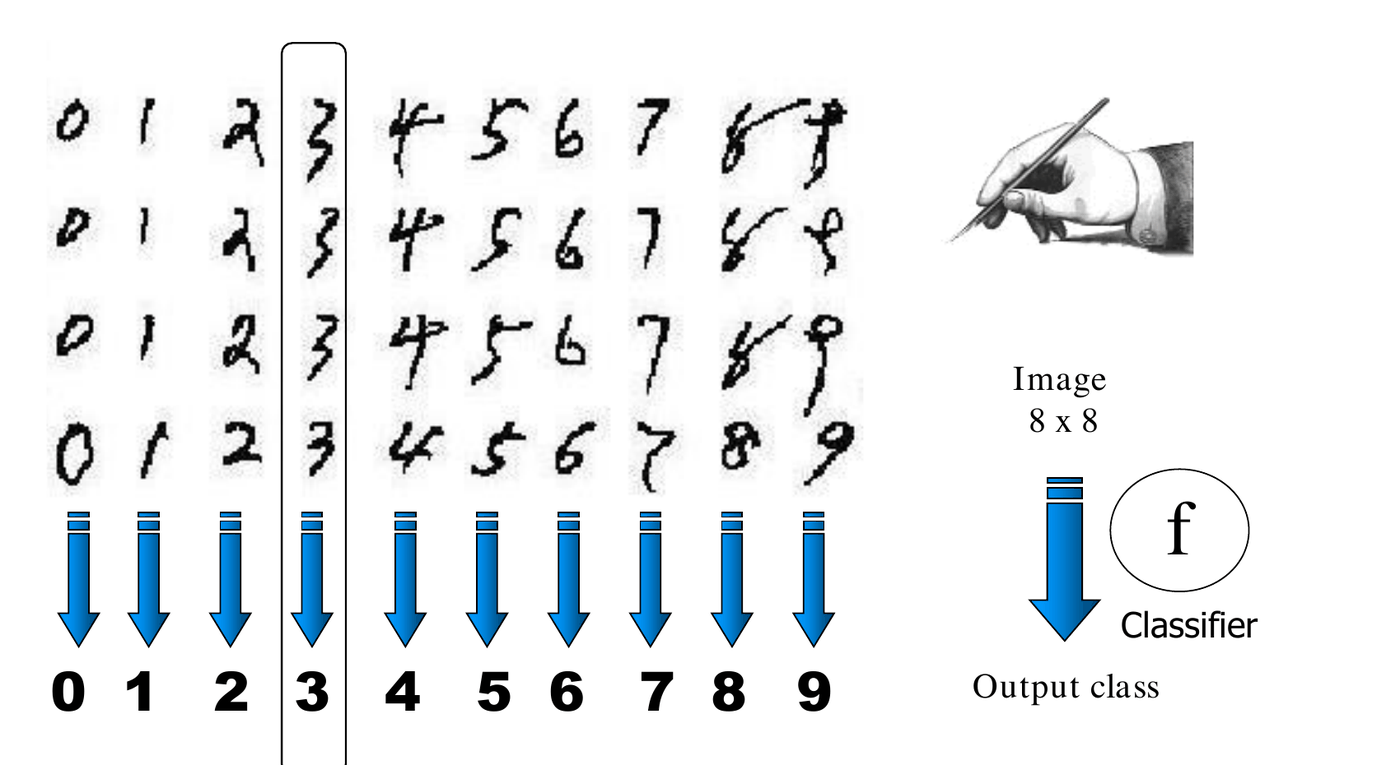
\includegraphics[width=0.80\linewidth,height=0.42\textheight,keepaspectratio]{images/01-intro_cifre-manoscritte.png}
\caption{Handwritten digit recognition: the classifier \(f\) maps an 8×8
image to the output class.}
\end{figure}

\subsection{Application areas}\label{aree-applicative}

ML is now pervasive in real systems (from OCR to human--machine
interfaces and search engines) and is the core of an interdisciplinary
area that since the 1980s has included:

\begin{itemize}
\tightlist
\item
  \textbf{Pattern Recognition} (face and speech recognition),
  \textbf{Computer Vision}, \textbf{Natural Language Processing} (from
  text classification to speech processing up to generative AI);
\item
  \textbf{Robotics}, adaptive systems and filters, intelligent sensor
  networks, personalised components;
\item
  \textbf{Knowledge Discovery and Data Mining}, Information Retrieval,
  analysis of complex data (medicine, biology, chemistry, web,
  marketing), financial forecasting.
\end{itemize}

In some fields --- NLP, Pattern Recognition, Computer Vision --- the
impact has been revolutionary, so much so that people speak of a ``new
AI''.

\subsection{Some recent successes}\label{alcuni-successi-recenti}

The professor shows some emblematic results:

\begin{itemize}
\tightlist
\item
  \textbf{Face recognition (DeepFace, CVPR 2014)}: combining deep
  neural networks and other ML techniques, trained on four million
  images of more than 4000 people, the system decides whether two
  photos depict the same person with 97.25\% accuracy, just below human
  accuracy (97.53\%).
\item
  \textbf{AlphaGo (DeepMind, March 2016)}: defeats the world Go
  champion.
\item
  \textbf{Medicine}: a deep neural network for skin cancer
  classification, trained on 130,000 cases (more than a doctor sees
  ``in many lifetimes''), reaches the accuracy of board-certified
  dermatologists (\emph{Nature}, 2017). At CIML in Pisa, the BrAID
  project applies AI to the diagnosis of Brugada syndrome.
\item
  \textbf{Machine translation}: Google Neural Machine Translation
  (since 2016) and DeepL (since 2017), entirely based on neural
  networks.
\item
  \textbf{Large Language Models and generative AI}: ChatGPT (OpenAI,
  November 2022), Bard/LaMDA (Google), open-source models such as Dolly,
  and systems that generate images (Stable Diffusion), video, music.
\item
  Autonomous driving, sensor data analysis, IoT.
\end{itemize}

ML provides the theoretical and methodological basis of the so-called
\emph{AI revolution}, with huge industrial investments. It is
considered a \textbf{GPT} (\emph{General-Purpose Technology}): a
technology capable of deeply transforming pre-existing economic and
social structures. The ``\emph{ML scientist}'' is among the most
sought-after profiles on the job market.

\begin{boxnote}{Turing Award 2018}

On 27 March 2019 the ACM awarded the Turing Award (the ``Nobel prize
of computing'') to \textbf{Yoshua Bengio, Geoffrey Hinton and Yann
LeCun} ``for conceptual and engineering breakthroughs that have made
deep neural networks a critical component of computing''.

\end{boxnote}

\begin{boxnote}{Nobel Prizes 2024}

In 2024 ML also reached the Nobel prizes: - \textbf{Physics}: to
\textbf{John Hopfield} and \textbf{Geoffrey Hinton} for foundational
discoveries and inventions that enable machine learning with artificial
neural networks (the Hopfield network as associative memory, the
Boltzmann machine). - \textbf{Chemistry}: to \textbf{Demis Hassabis}
and \textbf{John Jumper} (Google DeepMind) for protein structure
prediction with \textbf{AlphaFold}, and to \textbf{David Baker} for
computational protein design. Hassabis: \emph{``I've always thought
that if we could build AI in the right way, it could be the ultimate
tool to help scientists explore the universe around us.''}

\end{boxnote}

\subsection{The ultimate goal}\label{lo-scopo-ultimo}

Anything powerful can be dangerous if misused, but the ultimate goal
of AI and ML is to \textbf{benefit people} by solving problems big and
small, to \textbf{accelerate human progress} and to provide
intelligence to every other scientific field: augmenting our
capabilities while enhancing our humanity (P. Domingos,
\emph{Scientific American}, 2018).

\section{Why study Machine
Learning}\label{perchuxe9-studiare-il-machine-learning}

Within the master's degree, ML serves to:

\begin{itemize}
\tightlist
\item
  learn the \textbf{basic principles of learning processes}, from a
  computational point of view;
\item
  learn \textbf{new computing paradigms}, such as \textbf{neural
  networks}: studied as a computational paradigm since the 1940s with
  neurobiological inspiration, today they are a set of powerful models
  for \textbf{function approximation} with predictive capabilities,
  supported by a solid theory (\emph{learning theory}), and they are
  the basis of \textbf{Deep Learning};
\item
  be able to \textbf{apply these models rigorously};
\item
  have the foundations for all subsequent AI courses.
\end{itemize}

\subsection{Modern ML}\label{il-ml-moderno}

ML has moved from being a \textbf{collection of heuristic methods}
(tricks coming from biology, statistics, neural networks, fuzzy
logic\ldots) to building \textbf{general conceptual frameworks}. A new
understanding of the principles governing learning processes has
emerged, with three important consequences:

\begin{itemize}
\tightlist
\item
  expressing different models in different mathematical or computer
  ``languages'' \textbf{does not change the principles};
\item
  different application fields \textbf{do not change the principles};
\item
  new technological advances \textbf{do not change the principles}.
\end{itemize}

\begin{boxtip}{The common thread of the course}

``Machine Learning'' proper is the \textbf{core of principles and
methods} for building flexible and powerful computational models from
data. Individual models change, principles remain: this is what is
really worth learning.

\end{boxtip}

\subsection{Three views of ML}\label{tre-punti-di-vista-sul-ml}

\begin{enumerate}
\def\labelenumi{\arabic{enumi}.}
\tightlist
\item
  \textbf{As an AI methodology} → building adaptive and intelligent
  systems.
\item
  \textbf{As statistical learning} (inference of hypotheses according
  to mathematical principles) → building powerful predictive systems
  for intelligent data analysis.
\item
  \textbf{As a computing method for innovative application areas} →
  using models as tools for complex, interdisciplinary problems.
\end{enumerate}

The course considers all of them, with a \textbf{critical approach}:
for the various methods, their limits and appropriateness of use are
discussed, with attention to the underlying principles. There are two
practical goals: learning to \textbf{develop new ML models} and
learning to \textbf{apply state-of-the-art methodologies} to problems
in other fields.

\section{Course information}\label{informazioni-sul-corso}

\subsection{Prerequisites and goals}\label{prerequisiti-e-obiettivi}

No course is strictly required: we start from scratch. However, the
typical background of a scientific bachelor's degree is needed:
\textbf{calculus} (functions, differential calculus), \textbf{matrix
notation and computation}, \textbf{elements of probability and
statistics}, \textbf{algorithms}.

The course introduces the principles and the critical analysis of the
main paradigms (models and algorithms, with a focus on neural networks)
for learning from data. Concepts are introduced progressively, from the
simplest approaches up to state-of-the-art models, within the
conceptual framework of modern ML: \textbf{learning functions from
examples}. The focus is on:

\begin{itemize}
\tightlist
\item
  critical analysis of the features relevant to the design and use of
  ML;
\item
  \textbf{rigorous experimental evaluation}: there is a big difference
  between \emph{using} ML tools and using them \emph{correctly};
\item
  computational aspects of learning systems.
\end{itemize}

\subsection{Course structure}\label{struttura-del-corso}

The course has a strong structure: it starts from simple models and
arrives at the state of the art, and fundamental concepts are
introduced through different models. The practical advice is twofold:
(1) study the individual methods, (2) look for the \textbf{connections
and comparisons} among them, so as to abstract the concepts. The common
thread is understanding the relationship between \textbf{model
flexibility} and \textbf{complexity control}, a fundamental concept for
the ability to \textbf{generalise}.

\begin{figure}[htbp]
\centering
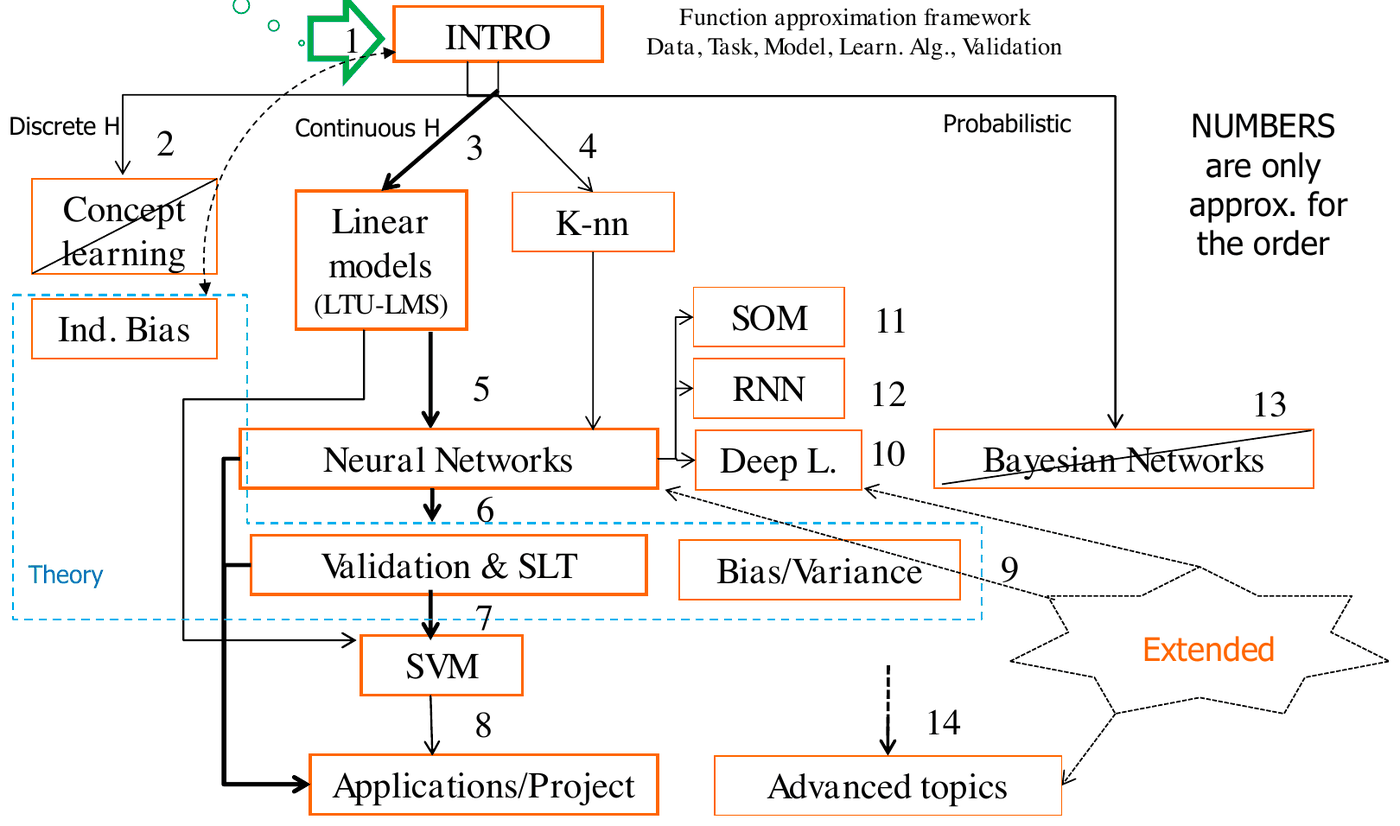
\includegraphics[width=0.93\linewidth,height=0.42\textheight,keepaspectratio]{images/01-intro_struttura-corso.png}
\caption{Map of the course. Numbers roughly indicate the order of the
lectures; the dashed ``Theory'' box groups the theoretical parts.}
\end{figure}

The map is not just an ordering of the lectures: it describes the path.
\textbf{``Building blocks''} (intermediate concepts and models) are
introduced and then composed to build ML models --- for instance,
neural networks are built from linear models, and a complete ML system
is built from validation techniques. For this reason the intermediate
models should be seen as pieces of a puzzle that comes together at the
end.

\begin{boxnote}{Order of lectures according to the map}

\begin{enumerate}
\def\labelenumi{\arabic{enumi}.}
\tightlist
\item
  Introduction (data, task, model, learning algorithm, validation) ---
  within the framework of \textbf{function approximation}.
\item
  Concept learning and inductive bias (discrete hypothesis space).
\item
  Linear models (LTU, LMS) (continuous hypothesis space).
\item
  K-nearest neighbors.
\item
  Neural networks.
\item
  Validation and Statistical Learning Theory.
\item
  Support Vector Machines.
\item
  Applications and project.
\item
  Bias/Variance.
\item
  Deep Learning (and, as an extension, SOM, RNN). 11--14. SOM, RNN,
  (Bayesian Networks --- removed from the syllabus), advanced topics
  (structured data).
\end{enumerate}

\end{boxnote}

The density of the course is not uniform: the introduction is slow and
``soft'', the core (neural networks, SVM, validation) is dense and
sequential, the advanced part is fast but less dense. The (optional)
project is announced roughly halfway through the course.

\subsection{Practical organisation}\label{organizzazione-pratica}

\begin{itemize}
\tightlist
\item
  \textbf{Lecturer}: Prof.~Alessio Micheli (Department of Computer
  Science), full professor, head of the CIML group
  (\emph{Computational Intelligence \& Machine Learning}) with more
  than 25 years of research in ML/AI, \textbf{president of the European
  Neural Network Society} (annual ICANN conference), co-founder of the
  IEEE Task Force on Reservoir Computing, associate editor of IEEE TNNLS
  and \emph{Neural Networks}. Goal of the course: to introduce current
  ML in 3 months, also retracing its foundations and history.
\item
  \textbf{Lectures} (A.Y. 2026/27): Tuesday, Wednesday and Thursday
  16--18, Room E. Lectures start on time so that there can be a break.
\item
  \textbf{Q\&A} with the lecturer: on Tuesday after the lecture
  (optional time, not part of the lecture) plus some special Q\&A
  lectures. For personal questions, write an email with the tag
  \textbf{{[}ML-26-Q{]}} in the subject (mandatory).
\item
  \textbf{Announcements}: via Teams and/or Moodle news. Lecture
  \textbf{recordings} are on Teams (\emph{Shared} tab →
  \emph{Recordings}); official lectures are in person only, streaming
  is informal and without guaranteed interaction.
\item
  \textbf{Make-up lectures}: on Monday afternoons (announced when
  needed) and in the recovery period from 9 to 18 December 2026 (to be
  taken into account before planning Christmas holidays). The lectures
  of 15--17 September 2026 did not take place and will be made up.
\end{itemize}

\begin{boxnote}{For those joining the course late}

All information is on the course \textbf{Moodle}
(elearning.di.unipi.it, with self-enrolment through the Unipi account):
slides, bibliography and \textbf{FAQ} section. It is also worth using
Teams (news and recordings) and classmates' notes. The project and the
practice tests are \textbf{not mandatory} for the exam. Do not ask the
lecturer about things already covered in the FAQ or in the first
lecture.

\end{boxnote}

\subsection{Exam}\label{esame}

\begin{boxwarning}{Updated rules (A.Y. 2026/27)}

The exam rules have changed compared to previous years: the
\textbf{project is no longer mandatory} and the exam is based on a
\textbf{mandatory written test}, with an oral exam only if needed.

\end{boxwarning}

The exam consists, in chronological order, of four phases.

\textbf{1. Practice tests during the course (optional).} At the end of
each cycle of lectures, short and simple practice tests are proposed on
Moodle. They serve for \textbf{self-assessment} (like homework
exercises, with a score that however \textbf{does not count for the
exam}), help keep up with the lectures and are evidence of active
participation. They have a deadline (typically one week), but if you
miss some you can continue the series. They prepare for the written
test, although format, content and depth are different. They are
announced only in class and with a short message on Teams.

\textbf{2. Project (optional).} At the end of the course (December) a
project can be carried out:

\begin{itemize}
\tightlist
\item
  group work of \textbf{2 students}, no exceptions;
\item
  content: implementation, application and/or analysis of an ML/neural
  network method or technique with \textbf{experimental evaluation}
  (projects coordinated with the CM course are possible);
\item
  format: public presentation of a \textbf{poster} in class (one of the
  last lectures), plus delivery of the developed material; there is a
  prize for the best poster;
\item
  after the presentation the exam can be taken in any session, but to
  discuss the project the two group members must take the exam
  \textbf{in the same session}.
\end{itemize}

The advice is not to apply for the project before having studied the
course contents thoroughly. Details will be given in a dedicated
lecture.

\textbf{3. Written test (mandatory).} It takes place after the course,
in the exam sessions (from January and February):

\begin{itemize}
\tightlist
\item
  it is mandatory to \textbf{register} for the exam on esami.unipi.it
  by the deadline (check it well in advance) and to cancel the
  registration if you decide not to attend;
\item
  it takes place \textbf{in person only}, in the classroom, on the
  date, time and room indicated on esami.unipi.it; not showing up is
  equivalent to withdrawing from that session;
\item
  questions must be answered on \textbf{pre-printed sheets} with space
  for free-form answers; bring a pen or pencil;
\item
  answers require \textbf{equations, drawings and/or descriptive parts}
  (quizzes and open questions);
\item
  no course or external material may be used, nor any electronic aid
  (virtual assistants, chatbots\ldots): the use of any device (laptops,
  smartphones, smart bands, earphones, smart glasses\ldots) is
  forbidden, under penalty of exclusion.
\end{itemize}

\textbf{4. Oral exam (only if needed) and grade registration.} Access
to the oral exam requires a sufficient level in the written test (the
list of admitted students is published on Moodle). The oral exam is
held in the same session as the written test, in person, typically in
the lecturer's office: in the days following the grading, the lecturer
assigns a slot to each student or group. If needed (depending on the
outcome of the written test), the oral exam is an interview on
\textbf{the whole syllabus} and may include discussion of the written
test and of the project. Special needs (priority, inability to attend
in person\ldots) are evaluated case by case upon request.

\begin{boxabstract}{Summary of the rules}

The evaluation takes into account: \textbf{result of the written test}
+ active participation (including tests during the course) + optional
extra activities (project, voluntary presentations at the end of the
course) + a possible full oral exam, if requested by the lecturer.

\begin{itemize}
\tightlist
\item
  \textbf{Sufficient} written test → in a slot a few days later:
  possible oral exam and \textbf{grade proposal} → if accepted,
  registration.
\item
  \textbf{Insufficient} written test or grade not accepted → repeat in
  a later session, chosen among the many during the year.
\end{itemize}

Completing 80\% of the online tests and a very good project may give a
\textbf{small bonus} (if the written test is already sufficient or
good), but they are \textbf{not necessary} either to take the exam or
to obtain the maximum grade. The key indicator is the \textbf{final
knowledge of ML and its depth}.

\end{boxabstract}

\begin{boxtip}{The professor's advice}

\begin{itemize}
\tightlist
\item
  Follow the lectures using the slides as a guide and study
  progressively during the course; Q\&A lectures are a discussion
  forum: this is a class, not a set of recordings.
\item
  First \textbf{study the course contents}, then work on the project:
  it increases both the effectiveness and the efficiency of the work.
\item
  If something is unclear: don't panic, ask the lecturer (Q\&A),
  collaborate with classmates, use books and papers (bibliography and
  personal research) and the course support tools. ML is a
  continuously evolving field: it must be studied!
\end{itemize}

\end{boxtip}

\subsection{Materials and bibliography}\label{materiale-e-bibliografia}

The main reference is the course slides (on Moodle, often published in
advance; make sure to use the latest version of the
\texttt{ML-26…-v*} files), which however must be complemented with
your own notes (the slides alone may not be enough to reconstruct the
thread of the lecture) and with books. The lecturer is willing to share
students' notes on Moodle. The main textbooks are:

\begin{itemize}
\tightlist
\item
  S. Haykin, \emph{Neural Networks and Learning Machines}, Prentice
  Hall, 3rd ed., 2008;
\item
  T. M. Mitchell, \emph{Machine Learning}, McGraw-Hill, 1997;
\item
  I. Goodfellow, Y. Bengio, A. Courville, \emph{Deep Learning}, MIT
  Press, 2016 (free online).
\end{itemize}

Other useful references: Russell--Norvig (\emph{AIMA}),
Hastie--Tibshirani--Friedman (\emph{The Elements of Statistical
Learning}, free copy online), Cherkassky--Mulier, Bishop
(\emph{Pattern Recognition and Machine Learning}, now \textbf{free}
from the publisher's website; and \emph{Neural Networks for Pattern
Recognition}), Duda--Hart--Stork, Shalev-Shwartz--Ben-David
(\emph{Understanding Machine Learning}, free online).

For \textbf{software libraries}: F. Chollet, \emph{Deep Learning with
Python}; A. Géron, \emph{Hands-on Machine Learning with Scikit-Learn,
Keras \& TensorFlow}; A. Zhang, Z. Lipton, M. Li, A. Smola, \emph{Dive
into Deep Learning} (Cambridge University Press, 2023, free online,
with examples in PyTorch, NumPy/MXNet, JAX and TensorFlow). The main
libraries will be introduced later by the course assistant. Beware:
there are a great many technical books and blogs, and one must pay
attention to scientific quality.

\begin{boxnote}{Course support}

\begin{itemize}
\tightlist
\item
  A \textbf{course assistant} to help with the development of the
  project (to be confirmed).
\item
  An experimental \textbf{tutor chatbot} (based on ChatGPT) for the ML
  2026 course: it helps clarify doubts, deepen concepts and get
  guidance on slides, definitions and exercises, always based on the
  official course materials. Details and links will be published in
  the Moodle news.
\end{itemize}

\end{boxnote}

In parallel, the course \textbf{Computational Mathematics for Learning
and Data Analysis} (CM) is very useful, as it provides the deep
mathematical foundations of learning methods (it is not, however,
mandatory for following ML).

\section{Mathematical background}\label{richiami-matematici}

To follow the course some basic concepts are needed: multivariable
calculus (partial derivatives, gradient), probability (densities, mean,
variance, normal distribution, conditional and joint probabilities),
matrix calculus (dot product, inverse, norms). Topics such as the
linear least-squares problem with the SVD and Lagrange multipliers can
be studied in parallel. Recommended references: appendix A of AIMA,
chapters 2--4 of the \emph{Deep Learning book}, and \emph{Mathematics
for Machine Learning} (2020).

The notation used is: \(x\) scalar, \(\mathbf{x}\) vector, \(X\)
matrix.

\subsection{Dot product and norms}\label{prodotto-scalare-e-norme}

\begin{boxdefinition}{Dot product (\emph{inner/dot product})}

\[
\mathbf{a} \cdot \mathbf{b} = a_1 b_1 + a_2 b_2 + \dots + a_n b_n = \sum_{i=1}^{n} a_i b_i = |\mathbf{a}|\,|\mathbf{b}| \cos\theta
\]

Equivalent notations:
\(\mathbf{a}\cdot\mathbf{b} = \mathbf{a}^T\mathbf{b} = \mathbf{a}^t\mathbf{b} = \langle \mathbf{a}, \mathbf{b}\rangle\),
and even just \(\mathbf{ab}\) if the context is clear.

\end{boxdefinition}

The relation with the cosine gives the geometric intuition: the dot
product measures \textbf{how much two vectors point in the same
direction}. It is maximal when they are parallel, zero when they are
orthogonal, negative when they point in opposite directions. This
reading will come up again and again (for example in linear models,
where \(\mathbf{w}^T\mathbf{x}\) measures the ``alignment'' of the
input with the weights).

The \textbf{Euclidean norm} (modulus, length) of a vector is \[
\|\mathbf{x}\|_2 = \sqrt{\mathbf{x}^T\mathbf{x}} = \sqrt{\sum_i x_i^2} = d(\mathbf{x}, \mathbf{0}),
\] often written simply as \(\|\mathbf{x}\|\) or \(|\mathbf{x}|\).
Other useful norms are the \textbf{\(L^1\) norm},
\(\|\mathbf{x}\|_1 = \sum_i |x_i|\), and the \textbf{max norm},
\(\|\mathbf{x}\|_\infty = \max_i |x_i|\).

More generally, an \textbf{inner product}
\(\langle \cdot,\cdot \rangle\) is a symmetric bilinear form that maps
a pair of vectors to a scalar: \[
\langle v, w\rangle = \langle w, v\rangle, \qquad \langle v+w, u\rangle = \langle v,u\rangle + \langle w,u\rangle, \qquad \langle kv, w\rangle = k\langle v, w\rangle.
\] The \textbf{Cauchy-Schwarz inequality} holds:
\(|\langle x, y\rangle| \le \|x\|\cdot\|y\|\) for all \(x, y \in V\).

\begin{boxnote}{Tensors}

A \textbf{tensor}, in the simplified view used in ML, is a
multidimensional array of numbers arranged on a regular grid with a
variable number of axes (for example \(X_{i,j,k}\) has 3 indices). In
ML it is used mainly as a notational convenience and to reason about
GPU computation; in mathematics tensors have richer properties (related
to changes of basis).

\end{boxnote}

\subsection{Partial derivatives and
gradient}\label{derivate-parziali-e-gradiente}

The \textbf{partial derivative} generalises the derivative to functions
of several variables: it is the derivative with respect to a single
variable, keeping all the others fixed. For \(f(x_1, x_2, x_3)\) one
computes \(\frac{\partial f}{\partial x_1}\),
\(\frac{\partial f}{\partial x_2}\),
\(\frac{\partial f}{\partial x_3}\).

\begin{boxdefinition}{Gradient}

The \textbf{gradient} of \(f\) is the vector of its partial
derivatives: \[
\nabla f = \operatorname{grad} f = \left( \frac{\partial f}{\partial x_1}, \dots, \frac{\partial f}{\partial x_n} \right) = \sum_{i=1}^{n} \frac{\partial f}{\partial x_i}\, \mathbf{e}_i
\] where the \(\mathbf{e}_i\) are the orthogonal unit vectors along the
coordinate directions.

\end{boxdefinition}

Its geometric meaning is fundamental for the whole course: at a point,
the gradient is a vector that \textbf{points in the direction of
steepest ascent}, and its norm indicates \textbf{how steep} the slope
is. The gradient therefore indicates where the function grows fastest,
while its opposite \(-\nabla f\) indicates the direction in which it
\textbf{decreases} fastest. This is exactly the idea behind
\textbf{gradient descent}, which we will use to train models by
minimising an error function.

\begin{figure}[htbp]
\centering
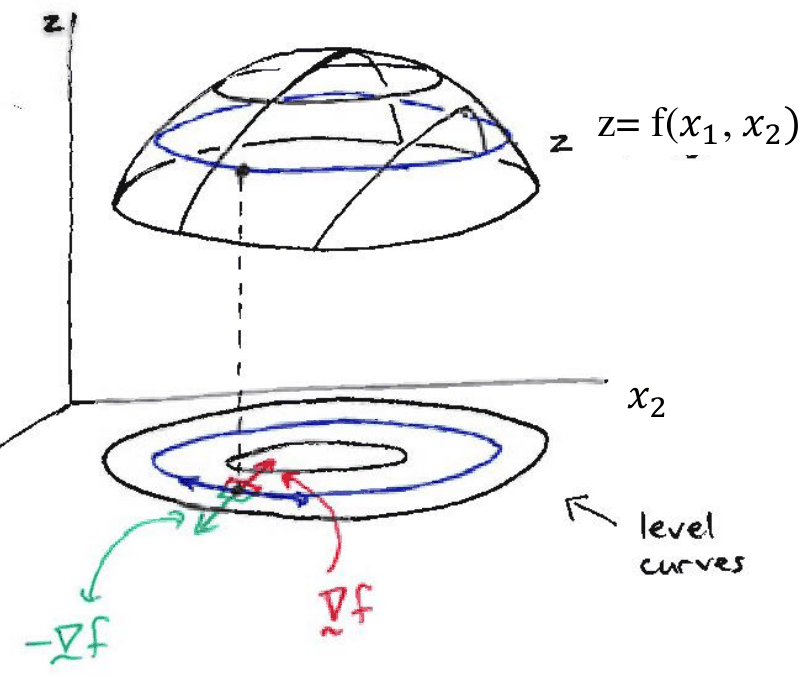
\includegraphics[width=0.47\linewidth,height=0.42\textheight,keepaspectratio]{images/01-intro_gradiente-superficie.png}
\caption{Gradient on a surface: \(\nabla f\) points towards the increase
of \(f\), \(-\nabla f\) towards its decrease; both are perpendicular to
the level curves.}
\end{figure}

A point where the gradient is zero is called a \textbf{stationary
point}. It can be a local minimum, a local maximum or a saddle point: a
zero gradient alone is not enough to tell which case it is.

\begin{figure}[htbp]
\centering
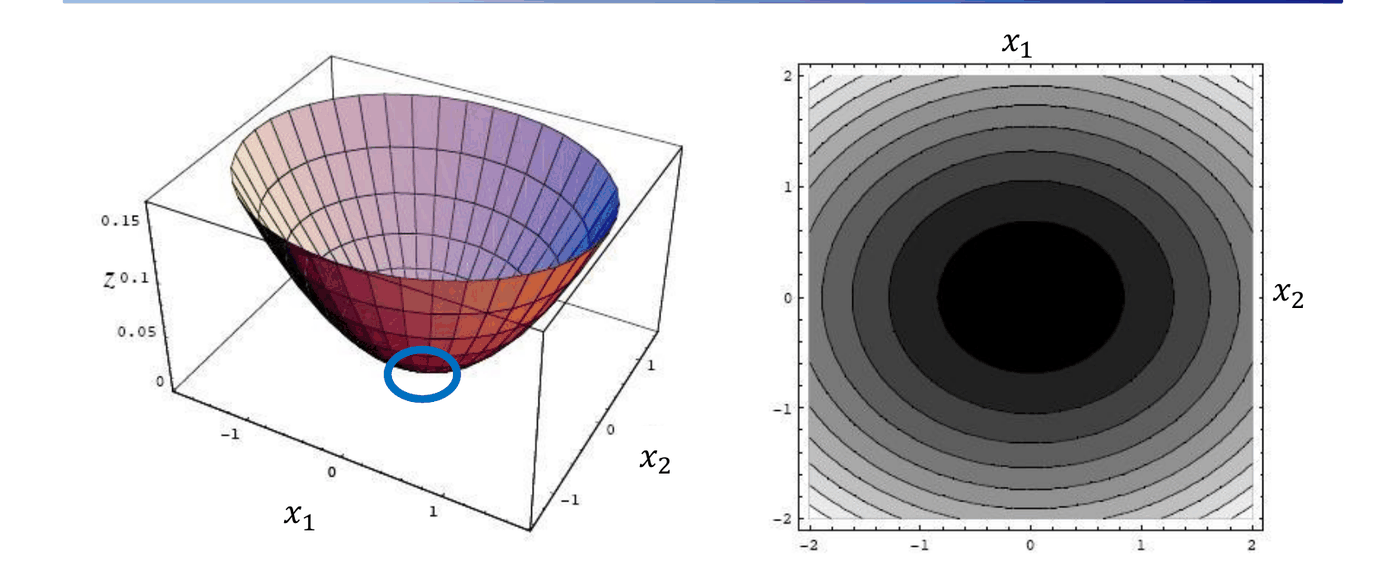
\includegraphics[width=0.80\linewidth,height=0.42\textheight,keepaspectratio]{images/01-intro_minimo-locale.png}
\caption{A minimum: at the lowest point of the paraboloid the gradient is
zero.}
\end{figure}

\subsection{Probability density: the
Gaussian}\label{densituxe0-di-probabilituxe0-la-gaussiana}

The \textbf{normal distribution} with mean \(\mu\) and variance
\(\sigma^2\) has probability density (the ``Gaussian function'') \[
f(x) = \frac{1}{\sigma\sqrt{2\pi}}\, e^{-(x-\mu)^2 / (2\sigma^2)}.
\] With \(\mu = 0\) and \(\sigma^2 = 1\) we obtain the \textbf{standard
normal}.

\begin{figure}[htbp]
\centering
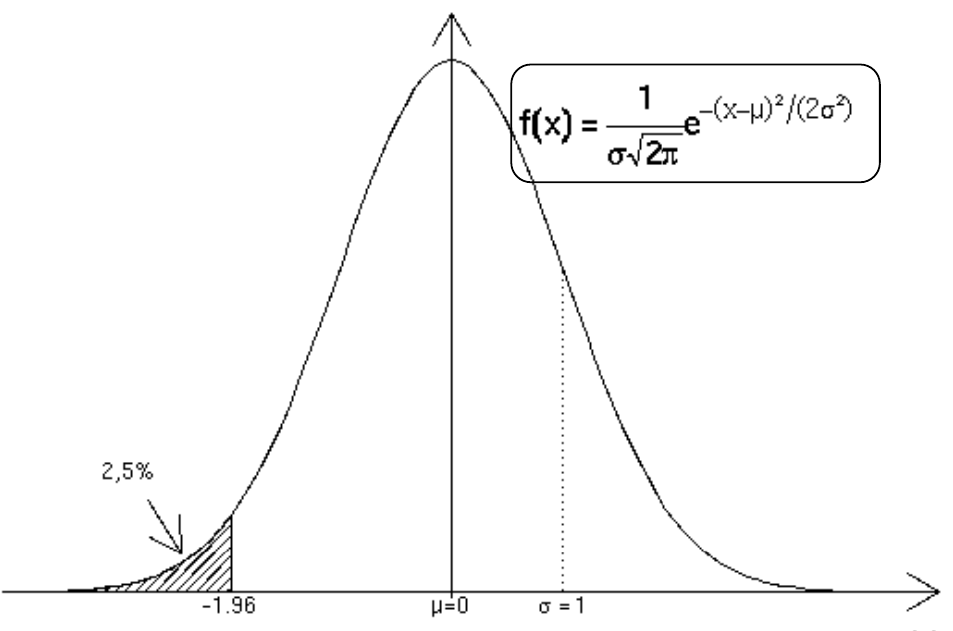
\includegraphics[width=0.57\linewidth,height=0.42\textheight,keepaspectratio]{images/01-intro_gaussiana.png}
\caption{Density of the standard normal: the area to the left of
\(-1.96\) is 2.5\%.}
\end{figure}

\section{Summary and next steps}\label{sintesi-e-prossimi-passi}

\begin{boxabstract}{Summary}

ML is the automatic learning of a task from examples: it is necessary
when data are abundant but explicit rules are missing. The course
approaches it as \textbf{function approximation from examples},
building models through successive ``building blocks'', paying
attention to the principles (which do not change as models change) and
to rigorous evaluation. The key concept running through the whole
course is the trade-off between \textbf{model flexibility} and
\textbf{complexity control}, on which \textbf{generalisation} depends.

\end{boxabstract}

The following lectures complete the introduction: lectures 2--3 cover
the usefulness of ML, learning as function approximation with a guiding
example, and the design components of an ML system (task, hypothesis
space, inductive bias, loss function, generalisation); lecture 4 goes
deeper into generalisation and validation.

\begin{boxquestion}{Possible exam questions}

\begin{itemize}
\tightlist
\item
  Why is ML a necessity and not a luxury? Under which conditions is it
  appropriate to use it?
\item
  What is the gradient and why does \(-\nabla f\) indicate the
  direction of steepest descent?
\item
  What is a stationary point? Is it always a minimum?
\end{itemize}

\end{boxquestion}
